
\documentclass[11pt]{article}

\usepackage{verbose_mdframed}

\makeatletter
\newcommand{\unchapter}[1]{%
  \begingroup
  \let\@makechapterhead\@gobble % make \@makechapterhead do nothing
  \chapter{#1}
  \endgroup
}
\makeatother


\begin{document}

\roundhomework{Graphical Modelling Guided Study}{}{}{ {\bf Updated:} 7.4.2023}
%\boxsection*[\LARGE Preface]
\section*{Preface}

\begin{itemize}
    \item Exercises are presented with omissions, solutions are unverified 
    \item Proofs are similarly good-faith efforts but unverified 
    \item \textcolor{red}{Red text} indicates my personal questions, lapses in understanding, or otherwise shakey areas 
    \item Other nice treatments of similar material include:
    \begin{itemize}
            \item Frederic Koehler's lecture on Common Gaussian Graphical Models \url{https://www.youtube.com/watch?v=V6NMDZB6LI4}
        	\item -- Illinois lecture note on graphical models class: \url{http://swoh.web.engr.illinois.edu/courses/IE598/info.html}
    \end{itemize}
    \item Useful\footnote{Not a pre-req (or any area of experience for me) but relevant optimization tools do crop up in Ch. 17 of ESL} references/notes on convex optimization and sub-gradient notation 
    \begin{itemize}
            \item Ryan Tibshirani's Convex Optimization Notes at \url{https://www.stat.cmu.edu/~ryantibs/convexopt/}
            \item Boyd and Vandenberghe's 2008 Textbook on Convex Optimization \url{https://web.stanford.edu/~boyd/cvxbook/bv_cvxbook.pdf}
    \end{itemize}
\end{itemize}

\section*{Non-Urgent/Of-Interest Review}

\begin{itemize}
    \item Community-Based Group Graphical Lasso (Pircalabelu, 2020) \url{https://www.jmlr.org/papers/volume21/19-181/19-181.pdf}
    \item Applications of lasso/grouped lasso (Friedman 2010) \url{https://www.asc.ohio-state.edu/statistics/statgen/joul_aut2015/2010-Friedman-Hastie-Tibshirani.pdf}
    \item Elastic net model selection in undirected graphica models (Cucuringu 2011) \url{https://arxiv.org/abs/1111.0559}
\end{itemize}


\newpage 

%\boxsection*[\LARGE To Do ]
\section*{To Do}

\subsection*{Important}

\begin{itemize}
    \item Review restricted strong convexity proofs 
    \begin{itemize}
        \item OLS with $\ell_1$ penalty (i.e. lasso) with 1) exact sparsity and 2) "partial" sparsity (i.e. $\mathbb{B}_q$ work, assumed sparsity)
        \item Understand how restricted eigenvalue condition implies restricted strong convexity 
    \end{itemize}
    \item GLM's (see section 6 in v1 of paper on ar$\chi$iv)
    \begin{itemize}
        \item For general link function but notably for logit link
        \item Note requirement of the tolerance function $\tau(\theta^*)$, the cause and how it alters the proof 
    \end{itemize}
\end{itemize}


\subsection*{Supplementary}

\begin{itemize}
    \item Implement Graphical Lasso (ESL Exercise 17.8)
    \item Review Wasserman Ch 19 (log-linear models)
    \item Review proofs:
    \begin{itemize}
    	\item Hammersley-Clifford theorem (iff/bi-directional)
	    \item Markov Properties  
        \begin{itemize}
            \item Global $\Leftrightarrow$ Pairwise $\Leftrightarrow$ Local (for positive distributions)
            \item Global $\Rightarrow$ Local $\Rightarrow$ Pairwise (generally)
        \end{itemize}
    \end{itemize}
    \item Review Junction-Tree Algo (ESL Ch 17) 
\end{itemize}

\newpage 
\section*{Misc. Proofs}

\subsection*{Hammersley-Clifford Theorem}

\subsection*{Equivalence of Pairwise and Global Markov Factorizations of Graph}


\newpage 

\begin{tcolorbox}
\vspace{4mm}
\bf \LARGE \chapter{Publications}
\vspace{4mm}
\end{tcolorbox}

\section*{Chen (2014): {\large \it Selection and Estimation for Mixed Graphical Models}}

\subsection*{Takeaways/High-Level Notes}
	\begin{itemize}
		\item This paper extends previous work to allow for estimation of conditional dependencies/associations within graphs of mixed distributions within the exponential family. Previous work focused on Gaussian graphs and more recently within 
		\begin{itemize}
			\item One related/contemporaneous work allowed for a mixed model of two distributions, this work allows for any(?) combination of the specified exponential family distributions
        \end{itemize}
	\end{itemize}

\subsection*{Further Review}
	
	\begin{itemize}
		\item Work through derivations of Ex. 1 to 4 (parameterization of conditional densities $p(x_s | x_{-s})$ in the proposed conditional density form (3))
        \begin{itemize}
            \item -- See \url{http://www.cs.cmu.edu/~epxing/Class/10708-16/note/10708_scribe_lecture10.pdf}
        \end{itemize}
        \item Revisit equation (3) (pg 3), how was this derived or arrived at? Is this a known extension of the exponential family definition in the graphical setting? 
		\item Review proofs in Appendix 
	\end{itemize}

\subsection*{Notes/Questions}
	
	\begin{itemize}
	
		\item The Introduction mentioned papers from \(\sim\)2009-13 that proposed semi-/non-parametric methods for conditional dependence estimation (Graphical Random Forest; Joint Additive Models) but criticizes these methods' efficiency. Is non-parametric estimation still an open research area?  
		
		\item What are these node potential functions, $f(x_s)$? Are they present to capture/account for the marginal "densities"(?) of a given random vector/node $x_s$? I want to understand because they seem to define the importance of $\alpha_s$, which in turn are parameters that we assume are known in the algorithm proposed in Section 3. Just trying to understand 1) what we are estimating in estimating $\alpha_{s1}$ and how strict (or just what the) assumption is when we say $\alpha_{sk}$ are known for $k\geq 2$
		\begin{itemize}
            \item The $\alpha_s$ are defined as $f(x_s) = \alpha_{s1}x_s + \alpha_{s2}x_s^2/2 + \sum \alpha_{sk}B_{sk}(x_k)$. That is, the $\alpha_s$ vector are coefficients for some linear combination that defines the node potential function 
        \end{itemize}

		\item Why allow for different penalty $\lambda$ by node type? This was counterintuitive to me. We've assumed that our graph is undirected, or $\theta_{st}=\theta)_{ts}$. However if $x_s, x_t$ are distributed differently (e.g. one Poisson and one binomial), $\not \Rightarrow \lambda_s \theta_{st}= \lambda_t \theta_{ts}$ (we could apply different optimal $\lambda$ values
		
		\item General question: Neighbourhood selection (and Graphical Lasso) are defined on $\ell_1$ penalty alone. Are there extensions (and if so, are they popular/open reserach) on $\ell_2$ or combined penalties?
			\begin{itemize}
                \item Found a 2011 treatment of an elastic net model for undirected Gaussian undirected graphs out of Princeton at \url{https://arxiv.org/abs/1111.0559}
            \end{itemize}
			
		\item Very general question: How (If you do) do you pick out useful techniques from some of the dense theory? And how do you identify what is a necessary pre-requisite or where you can assume or glance over some knowledge? For example, I don't have a convex optimization background outside of it's discussion in some stat theory (read: very little). So the proof of theorem 1 relying primal-dual witness method. Is this worthwhile to learn and how do I identify what is a useful/generalizable tool/skill and what may be useful just for this paper (and worth either accepting, or asking someone else to verify that I do know has this background)? 
	\end{itemize}
	
	
\newpage 

\section*{Wainwright (2012) {\large \it Unified Framework for High-Dimensional Analyais of $M$-Estimators with Decomposable Regulators}}

\subsection*{Further Review/Questions (9/6)}
\begin{itemize}
	\item{Where does equation 18 come from? I am familiar with explicit forms of the remainder in univariate expansions, but I'm not familiar with the multivariate remainder expression (and am unsure how this specific expression is derived)}
	\item End of page 12, how does this correspond to a restricted eigenvalue condition? 
\end{itemize}

Applications to Lasso (4-5):

\begin{itemize}
	\item 4.1) For least squares LASSO ($\ell_1$ penalty), the Taylor series involved in the RSC definition is exact, and thus independent of $\theta^*$ (the parameter's true value for all intents and purpose). This, combined with the definition of the cone set $\mathcal{C}$ to which $\hat{\Delta}$ must belong simplifies the necessary RSC demonstration into a restricted eigenvalue condition, which can be shown to be met with high probability for Gaussian (and subGaussian) design matrices (even with dependencies)
    \begin{itemize}
        \item But no comments yet on convergence, accuracy, etc. just meeting this RSC definition as necessary for further analysis of this M-estimation problem 
    \end{itemize}
    \item 4.2) Assume RE to assume RSC. We know $\ell_1$ is decomposable. Thus we have the bounds from Corollary 1 on the error vector, we must simply identify the regularization constant $\lambda_n$ and the compatibility function $\Psi(M)$ for $\mathcal{R}(\cdot) = ||\cdot||_1$ and error norm $||\cdot||_2$ (which is the meat of the proof of Corollary 2, besides the implicit $RE \Rightarrow RSC$ argument that I believe 4.1 makes)
		\begin{itemize}
            \item Note the sub-gaussian (and normalizing) assumption allows for the high-probability argument made in the proof of corollary 2. 
        \end{itemize}
	\item 4.3) So assuming now $\theta^*$ is weakly sparse, that is not sparse but adequately-approximated by a sparse vector. We construct a set of sparse vectors for $\mathcal{M}$, and now have that $\theta^* \not\in \mathcal{M}$, leading to 1) this ball-shaped set and 2) the need for a positive tolerance function $\tau(\theta^*)$. This is contradicted however by the statement in Corollary 3 that $\theta^* \in \mathbb{B}_q(R_q)$, that is $\theta^*$ actually does belong to our model/sparsifiable set. 
	\begin{itemize}
        \item Maybe it's that $\theta^*$ belongs to $\mathbb{B}_q(R_q)$ but we are estimating with a truly sparse set (i.e. $\mathbb{B}_0(R_0)$ with at most $R_0$ non-zero features), a stricter condition/subset of the $\mathbb{B}_q$ sparsifiable set 
        \item GLM extension essentially (with exponential family requirement although this is w/in definition of GLM) is just a revisited Taylor Series expansion with analogous work and results and an additional\textcolor{red}{(?)} constraint that sample size scales in $\Omega(s \log p)$ for sparsity $|S|=:s$.
    \end{itemize}
\end{itemize}
\subsection*{Takeaways}


Definitions in section 2 as set-up for Theorem 1:
\begin{enumerate}
	\item Identifies a suitable bound on our penalty $\lambda_n$ related to the norm $\mathcal{R}(\grad \mathcal{L}(\theta^*))$ such that our errors $\delta$ for any optimal solution $\hat{\theta}$ are contained in a bounded cone (if $\theta^* \in \mathcal{M}$, a star-shaped set otherwise)
	\item Strong convexity of our loss function $\mathcal{L}$ is necessary to ensure that $|\mathcal{L}(\theta^*) - \mathcal{L}(\hat{\theta}_{\lambda_n}|$ approaching 0 implies that $\delta$ (or $\hat{\delta}$ is also small. We can be less strict in this assumption and only require strong convexity in a neighborhood about $\theta^*$, and in fact can focus on the cone (or star-shaped set) identified in definition 1, leading us to this RSC definition/consideration 
	\item \textcolor{red}{It seems intuitive to want some subspace compatibility measure, as we can construct any subspace $M$ (and norm, with decomposability as in Dfn 1) and $\overline{M}^\perp$ that we deem appropriate, but what is the idea behind this specific measure of compatibility? } My intuition is that this captures the interplay between the subspace $M$ (by suping over $u \in M$) and balancing the norm $\mathcal{R}$ with the 
\end{enumerate}

\begin{itemize}
	\item namely, a decomposability property for the regularizer and a notion of restricted strong convexity that depends on the inter- action between the regularizer and the loss function.
	\item Decomposability (want to ensure I understand this perturbation intuition): 
		\begin{itemize}
            \item Consider a model $M$ and our estimation $\overline{M}$ (for simplicity consider $M = \overline{M}$ but general result offered for $\overline{M} \subseteq M$. For $\theta \in M$ and $\gamma \in \overline{M}$, $\theta+\gamma$ (and specifically $\gamma$) can be considered deviations away from the model space 
        \end{itemize}
\end{itemize}

\subsection*{Questions/Notes}

	\begin{itemize}
		\item How do you best understand/learn the "history" of a given topic/method?
		\begin{itemize}
			\item Sometimes it frequently pops up and just sticks (Tibshirani 1996 key ex), either in coursework or a common "parent" publication across 
			\item "Review"-esque papers like this (or at least papers that provide succinct overviews of notable papers) are great but not always available
        \end{itemize}
        \item  How do we think about $\theta^* \in M$? Is this somewhat similar to identifiability? Like a well-specified model, such that $M$ our subspace which encodes the constraints (or other parameterizations/properties) that we believe are true for $\theta$ actually contains $\theta^*$ (analogous to "ground truth" in the frequentist univariate parameter estimation setting)
		\item {\bf More transparently, what is $\overline{M}$ in relationship to $M$?} Topological closures(?): Important to understand the distinction $\overline{M} \subseteq M$ and $\overline{M} = M$? I understand when we do not have equality (low-rank matrix estimation), but I don't necessarily understand what a topological closure is 
		\item (pg. 5-6) {\it "With certain exceptions, it is computationally expensive to enforce a rank-constraint in a direct manner..."} What are the issues? Something related to the number combinations of row/column combinations that could result in a specific rank become prohibitively large (even if considered cleverly)? 
		\item (pg. 11 (c)) How does the tolerance $\tau_\mathcal{L}$ related to unidentifiable components in a high-dim model? 
	\end{itemize}

\subsection*{Further Review}

	Pressing/Paper Material 
	\begin{itemize}	
		\item Figure 1 (3-dimensional error vector, geometric intuition behind $\mathbb{C}(M, \overline{M}^\perp, \theta)$ when $\theta^* \in M, \theta^*\not\in M$ respectively 
	\end{itemize}
	(Newly) Conceptual
	\begin{itemize}
		\item Review equivalency of lasso and basis pursuit de-noising
		\begin{itemize}
			\item See \url{https://www.cs.cornell.edu/courses/cs6220/2017fa/CS6220_Lecture21_2.pdf}
			\item {\it Possibly only of historical relevance}
        \end{itemize}
		\item Definition/abstraction of a (topological) closure:
		\begin{itemize}
			\item For subspace $M \subseteq \mathbb{R}^p, \left(M^\perp \right)^\perp \equiv \overline{M}$ is a closure of $M$ (more accurately is a closure operator on $M$) 
			\item With the exception of discussion of low-rank matrices and the nuclear norm, we can work with $M = \overline{M}$ and not concern ourselves with the concept of topological closures 
        \end{itemize}
		\item Prove (pg 7) dual-norm for group-norm (similar to $\ell_1 - \ell_\infty$ dual norm relationship proof)
	\end{itemize}
	
\subsection*{Misc (Somewhat) Related Work}

\subsubsection{Proof of equivalent dual-norm definitions}

WTS $\sup_{u \in \mathbb{R}^p\backslash\{0\} } \frac{\langle u, v \rangle}{\mathcal{R}(u)} = \sup_{\mathcal{R}(u)\leq 1} \langle u,v \rangle$

1) 

\begin{gather*}
	A := \{u : \mathcal{R}(u) \leq 1\} \subseteq \{u : ||u|| \leq 1, u \neq 0\} =: B 
	\\
	\Rightarrow 
	\sup_{\mathcal{R}(u)\leq 1} \langle u,v \rangle 
	\leq 
	\sup_{\mathcal{R}(u)\leq 1}\frac{\langle u,v \rangle}{\mathcal{R}(u)}
	\leq 
	\sup_{u \in \mathbb{R}^p\backslash\{0\} } \frac{\langle u, v \rangle}{\mathcal{R}(u)}
\end{gather*}

\newpage
\begin{tcolorbox}
\vspace{4mm}
\bf \LARGE \chapter{Elements of Statistical Learning}
\vspace{4mm}
\end{tcolorbox}

\section*{Chapter 17: Undirected Graphical Models}

%\subsection*{Questions, Notes, Properties, Definitions, etc. }


\subsection*{Overview/Intro}
\begin{enumerate}
    \item \textit{Omitting information that is shared with Wasserman chapters, which are more introductory than ESL's discussion of graphical algorithms}
    \item \textcolor{red}{\sout{We define clique potentials (similar to the Wasserman chapter) as affinities (affine functions?). Since we express the density function as product of clique functions, I assume these must be positive functions defined on each clique. Are there other constraints or definitions about these affinities?}}
    	\begin{itemize}
            \item -- My (still limited, possibly incorrect) understanding is that these are simply positive functions that are context-specific or user-defined. Wainwright/Jordan describes these as {\it compatibility functions} which are defined based on a model. 
    	    \item -- An example of a simple compatibility functions is a binary decision rule that is 0 for any configuration of vertices/values that occurs with probability 0, and 1 otherwise. That is for clique $(x_i, x_j, x_k)$ with known impossible configuration $(z_i, z_j, z_k)$, the compatibility function is equivalent to the boolean $\lnot z_i \lor \lnot z_j \lor \lnot z_k$.
        \end{itemize}
    \item Hammserley-Clifford: From ESL, states that we can equivalently represent the joint density function of a graph ($\mathcal{G} = (V,E)$) $f_V$ as a product of clique affinities {\bf for Markov networks with positive (i.e. non-zero) distributions}
    \begin{itemize}
        \item -- That is for set of maximal cliques\footnote{
            From Wainwright, Jordan (2008), I believe we can also use a set of non-maximal cliques (or any combination of cliques) in this factorization when convenient
            } $\mathcal{C}$ and graph $\mathcal{G} = (V, E)$, $f_\mathcal{G}(x) \propto \prod_{C \in \mathcal{C}}\psi_C (x_C)$
    \end{itemize}

    \item \textcolor{red}{Another question re: HC theorem/clique-factorization of the density function "implies a graph with independence properties defined by the cliques...". So this is true even with overlap in the maximal cliques (or within whatever cliques are used to factorize the density function)? }
        
    
\end{enumerate}

\subsection*{17.3 Continuous Variables}

\begin{itemize}
    \item Assuming a Gaussian distribution describing our nodes allows for some convenient estimation properties to arise in graph structure and/or parameter estimation:
    \begin{itemize}
        \item Generally (or perhaps vaguely), Gaussian graphical models allow estimation problems to be constructed conveniently as linear regression problems (see 17.3.1 for regression estimating equations, 17.3.2 for lasso regression for structure estimation)
        \item For $\mathbf{X} \sim N(\boldsymbol{\mu}, \boldsymbol\Sigma)$ and $\boldsymbol\Theta = \boldsymbol\Sigma^{-1}$, $\theta_{ij}=0 \Leftrightarrow X_i \perp X_j | \text{rest}$
    \end{itemize}
    \item \textcolor{red}{I assume the algorithm for graphs with completely known structure is a (almost prohibitively) rare setting for any utility. Are there also settings with partially specified structure? Suppose we know the existence/absence of some specific edges but otherwise have no other information? A hybrid of the structure-specified and -unspecified approach?}
\end{itemize}

\subsubsection{17.3.1 Estimating Equations for Graphs with Known Structure}

\textcolor{red}{\sout{Pg 631, authors claim {\it "The dependence of Y on Z in (17.6) is in the mean term alone"} for this conditional Gaussian relationship. How is this true? We also see this $\sigma_{XY}$ term in the Variance as well, where $\sigma_{XY}$ is the covariance of $Y, X$. }
}
The dependence on $Z$ is only in the mean. The variance term includes $\sigma_{ZY}$ which is a parameter/"constant" (i.e. does not vary by values of $Z$, just captures the dependence relationship between $Y, Z$.   \\


\textcolor{red}{See work/question for Exercise 17.5 for question of distinction between $W, S$ matrices in presented algorithm}

\subsubsection{17.3.2 Estimation of Graph Structure (Graphical Lasso) }

\textcolor{red}{I don't necessarily understand the difference between the initial 2006 lasso approach to structure estimation (fitting $p$ lasso models, arguing edge $\theta_{ij}$ exists iff $\beta_j$ is non-zero for $X_i$ regressed on $\mathbf{X}\backslash\{X_i\}$) and the algorithm described in 17.2 (graphical lasso). GL is  solving an equivalent system of equations, no? And this algorithm has guaranteed convergence pending lasso convergence. I would need to read the 2008 graphical lasso paper to undertand its theoretical guarantees and/or possible convergence issues
}

\subsection*{17.4 Discrete Variables}

\newpage 

\subsection*{Exercises}

\begin{enumerate}
\item 
    \begin{enumerate}[label=(\alph*)]
        \item Maximum Cliques:
        $\{X_1, X_2, X_3\}$
        , $\{X_1, X_4 \}$
        , $\{X_3, X_4 \}$
        , $\{X_5, X_6 \}$
        \item Conditional Independencies:
        Trivially, any $X_i, X_j$ without an edge is independent conditional on all other nodes\\ 
        By separation, a list (with some redundancies): \\  
        $X_1 \perp X_5 | X_6$ \\         
        $X_2 \perp X_{3,4} | X_1$
        $X_2 \perp X_6 | X_5$ \\ 
        $X_3 \perp X_{1, 2,5,6} | X_4$ \\
        $X_4 \And X_3 \perp X_{2,5,6} | X_1$ \\
        $X_5 \perp X_{1,2,3,4} | X_6$        
    \end{enumerate}

    
\item {\it Omitted }

\item 
    \begin{enumerate}[label=(\alph*)]
        \item 
        Note $\Sigma \in \mathbb{R}^{p \times p}$ can be partitioned as 
        
        \begin{align*}
            \Sigma = 
            \begin{bmatrix}
            \Sigma_{aa} & \Sigma_{ab} \\ 
            \Sigma_{ba} & \Sigma_{bb}
            \end{bmatrix}
        \end{align*}
        
        for $\Sigma_{aa} \in \mathbb{R}^{2 \times 2}; \ \Sigma_{ab}, \Sigma_{ba}^T \in \mathbb{R}^{2 \times p-2}; \ \Sigma_{bb} \in \mathbb{R}^{p-2 \times p-2}$. 
        
        We can partition $\Theta \equiv \Sigma^{-1}$ and use known properties of the inverses of partitioned matrices to demonstrate:
        
        \begin{gather*}
                \Theta 
                =
            \begin{bmatrix}
                \Theta_{aa} & \Theta_{ab} \\ 
                \Theta_{ba} & \Theta_{bb}
            \end{bmatrix}
                = 
                \Sigma^{-1}
                =
            \begin{bmatrix}
                \left( \Sigma_{aa} - \Sigma_{ab}\Sigma_{bb}^{-1}\Sigma_{ba} \right)^{-1} & f_2\left(\Sigma \right) \\ 
                f_3\left(\Sigma \right) & f_4\left(\Sigma \right)
            \end{bmatrix}
        \end{gather*}
        
        where we see $\Theta_{aa} = \Sigma_{a,b}^{-1}$.

    \item 
        \begin{align*}
            \Sigma_{a,b}
            &=
            \begin{bmatrix}
                Cov(X_1, X_1 | \text{rest})
                & Cov(X_1, X_2 | \text{rest})
                \\
                Cov(X_2, X_1 | \text{rest})
                & Cov(X_2, X_2 | \text{rest})   
            \end{bmatrix}
            \\
            &\Rightarrow 
            \Sigma_{a,b}^{-1}
            =
            \Theta_{aa}
            \propto 
            \begin{bmatrix}
                Cov(X_2, X_2 | \text{rest})
                & -Cov(X_1, X_2 | \text{rest})
                \\
                -Cov(X_2, X_1 | \text{rest})
                & Cov(X_1, X_1 | \text{rest})   
            \end{bmatrix}
        \end{align*}

        The off-diagonals of $\Theta_{aa}=0 \Rightarrow \rho_{1, 2|\text{rest}}=0$. Noting that we've selected $a,b$ such that $X_a=(X_1, X_2)$ as $j=1, k=2$ WLOG (i.e. the result holds $\forall j\neq k$) completes the argument.


    \item\footnote{Wikipedia actually has a nice  walkthrough of the calculation of the partial conditional correlation formula, at  \url{https://en.wikipedia.org/wiki/Partial_correlation\#Using_matrix_inversion}}
        We can (less lazily compared to 3b) calculate the partition of precision matrix $\Theta_{aa}$, where $\theta_{ij} = Cov(X_i, X_j | \text{rest})$: 

        \begin{align*}
        \Sigma^{-1}_{a,b}
        =
        \Theta_{a,b}
        &=
        \frac{1}{\theta_{ii}\theta_{jj} - \theta_{ij}^2}
        \begin{bmatrix}
            \theta_{jj}
            & -\theta_{ij}
            \\
            -\theta_{ji}
            & \theta_{ii}
        \end{bmatrix}
        \end{align*}

        Then 
        $\text{diag}(\Theta)^{1/2}
        =
        \begin{bmatrix}
        \frac{1}{\sqrt{\theta_{jj}}} & 0 \\
        0 & \frac{1}{\sqrt{\theta_{ii}}}
        \end{bmatrix}$ and: 


    \begin{align*}
        \mathbf{R}
        =
        \text{diag}(\Theta)^{-1/2}
        \cdot \Theta \cdot
        \text{diag}(\Theta)^{-1/2}
        &=
        \begin{bmatrix}
         \sqrt{\theta_{jj}} & -\frac{\theta_{ij}}{\sqrt{\theta_{jj}}} \\ 
         -\frac{\theta_{ji}}{\sqrt{\theta_{ii}}} & \sqrt{\theta_{ii}}
        \end{bmatrix}
        \begin{bmatrix}
        \frac{1}{\sqrt{\theta_{jj}}} & 0 \\
        0 & \frac{1}{\sqrt{\theta_{ii}}}
        \end{bmatrix}
    \\
        &= 
        \begin{bmatrix}
            1 
            & 
            -\frac{\theta_{ij}}{\sqrt{\theta_{jj}\theta_{ii}}} 
            \\ 
            -\frac{\theta_{ji}}{\sqrt{\theta_{jj}\theta_{ii}}} 
            & 
            1 
        \end{bmatrix}
    \end{align*}

    where we see $r_{ij} = \rho_{ij}|\text{rest}$ by definition of $\rho_{ij}|\text{rest} =-\frac{\theta_{ij}}{\sqrt{\theta_{jj}\theta_{ii}}}$. 
    \end{enumerate}

    
    \item 
    Notation: Let $\{X_3, X_4, ..., X_p\} = X^* = X_{3, ..., p}$: 
    
    \begin{align*}
        X_1 \perp X_2 | X^*
        &\Leftrightarrow 
        f_{X_1, X_2 | X^*} = f_{X_1 | X^*} f_{X_2 | X^*}
        \\
        f_{X_1, X_2 | X^*}
        &=
        \frac{
        f_{X_1, X_2, X^*}
        }{
        f_{X^*}
        }
        =
        \frac{
        f_{X_1 | X_2, X^*} f_{X_2|X^*}f_{X^*}
        }{
        f_{X^*}
        }
        \\
        &= f_{X_1 | X_2, X^*} f_{X_2 | X^*}
        \\ 
        &=
        f_{X_1 | X^*} f_{X_2 | X^*}
    \end{align*}


    \item 
    From 17.3.1 (and work below under Misc. Claims), the gradient of the log-likelihood for our Gaussian graphical model is 
    $\nabla \ell(\Theta; \mathbf{X}) = \Theta^{-1} - S$ (with $\Gamma = \mathbf{0}$, as all edges are known and present).  $S = \Theta^{-1}$ and assuming a similar partitioning scheme as in 17.3.1: 

    \begin{align*}
    S 
    = 
    \Theta^{-1}
    &\Rightarrow 
    \begin{bmatrix}
        S_{11} & s_{12} \\ 
        s_{21} & s_{11}
    \end{bmatrix}
        \begin{bmatrix}
        \Theta_{11} & \theta_{12} \\ 
        \theta_{21} & \theta_{22}
    \end{bmatrix}
    =
    \begin{bmatrix}
        \mathbf{I} & 0 \\ 
        0^T & 1
    \end{bmatrix}
    \\
    &\Rightarrow 
    S_{11}\theta_{12} + s_{12}\theta_{22} = 0
    \\
    &\Rightarrow 
    s_{12} 
    = 
    -\frac{
    S_{11}\theta_{12}
    }{
    \theta_{22}
    }
    =
    S_{11}\beta 
    \end{align*}
    
    \begin{align*}
        \Theta - S \stackrel{!}{=}0
        &\Rightarrow
        s_{11} - s_{12} = 0
        \Leftrightarrow 
        S_{12}\beta - s_{12} = 0 \qed 
    \end{align*}
    \textcolor{red}{This problem feels a bit weird. In order to use this substitution, the gradient gives us $s_{12} - s_{12}$, no? Which is trivially true. IN the 17.3.1 derivation, we use $W$. Not sure if I truly understand the distinction of $S, W$. }

    \item Omitted, result follow nearly immediately from 17.16 (or the provided 17.41-2) and a profile-likelihood style argument

    \item {\it Incomplete (Programming)} 

    \item {\it Incomplete (Programming)}

    \item 
\end{enumerate}

\begin{tcolorbox}
    \vspace{4mm}
    \Large \bf Misc. Claims, Proofs, Work
    \vspace{4mm}
\end{tcolorbox}

{\bf Claim:} The log-likelihood of $N$ random samples of a $k-$dimenisonal multivariate Gaussian with mean $\boldsymbol\mu$ and covariance matrix $\boldsymbol\Sigma = \boldsymbol\Theta^{-1}$ can be expressed as (noting $\mathbf{x} \in \mathbb{R}^k; \boldsymbol\Theta, \mathbf{S} \in \mathbb{R}^{k \times k}$) for sample covariance matrix $\mathbf{S} =  (\mathbf{x}-\mu)(\mathbf{x}-\mu)^T$:

\begin{align*}
    \text{WTS}
    \ell(\boldsymbol\Theta)
    &= \textcolor{red}{(\propto?)}
    \log \det \boldsymbol\Theta
    -
    \trace(\mathbf{S}\boldsymbol\Theta )
    \\
    \\
    \ell(\boldsymbol\Theta)
    &= 
    \sum_{i=1}^N
    \log\left[
    (2\pi)^{-k/2} 
    \det(\boldsymbol\Sigma)^{-1/2}
    \exp{
    -\frac{1}{2}
    (\mathbf{x}_i-\boldsymbol\mu)^T
    \boldsymbol\Sigma^{-1}
    (\mathbf{x}_i-\boldsymbol\mu)
    }
    \right]
\\
    &= 
    \sum_{i=1}^N
    \log\left[
    (2\pi)^{-k/2} 
    \det(\boldsymbol\Theta)^{1/2}
    \exp{
    -\frac{1}{2}
    (\mathbf{x}_i-\boldsymbol\mu)^T
    \boldsymbol\Theta
    (\mathbf{x}_i-\boldsymbol\mu)
    }
    \right]   
\\
    &\textcolor{red}{\propto}
    \log \det \boldsymbol\Theta 
    -\frac{1}{2}
    \sum_{i=1}^N
    (\mathbf{x}_i-\boldsymbol\mu)^T
    \boldsymbol\Theta 
    (\mathbf{x}_i-\boldsymbol\mu)    
\\
    &
    \stackrel{
    \overline{\mathbf{x}} = \hat{\mu}_{MLE}
    }
    {
    \textcolor{red}{\propto}
    }
    \log \det \boldsymbol\Theta 
    -
    \frac{1}{2}
    \sum_{i=1}^N
    (\mathbf{x}_i-\overline{\mathbf{x}})^T
    \boldsymbol\Theta 
    (\mathbf{x}_i-\overline{\mathbf{x}})   
\\
    &\textcolor{red}{\stackrel{?}{=}}
    \log \det \boldsymbol\Theta 
    -
    \trace(\mathbf{S}\boldsymbol\Theta) 
\end{align*}

\newpage 
\begin{tcolorbox}
\vspace{4mm}
\bf \LARGE \chapter{All of Statistics (Wasserman)} 
\vspace{4mm}
\end{tcolorbox}



\section*{Chapter 17: Directed Graphs}

\subsection*{Questions, Definitions, Notes, Properties, etc.}

\begin{enumerate}
    \item An \textbf{unshielded collider} is any collider whose "pointing nodes" are disconnected/non-adjacent:
    \begin{figure}[h]
    \centering 
    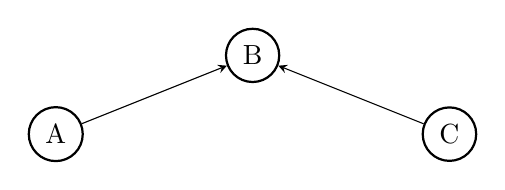
\begin{tikzpicture}
        \begin{scope}[every node/.style={circle, thick, draw}]
        \node (A) at (0,3) {A};
        \node (B) at (2.5,4) {B};
        \node (C) at (5,3) {C};
        \end{scope}

        \begin{scope}[>={stealth[black]}]
        \path [->] (A) edge node {} (B);
        \path [->] (C) edge node {} (B);
        \end{scope}
    \end{tikzpicture}
    \ is unshielded, whereas
    \end{figure}
    
    \begin{figure}[h]
    \centering
    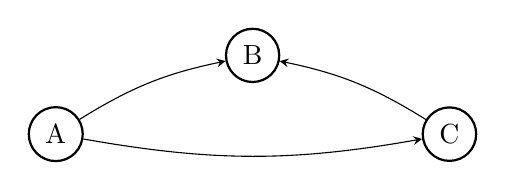
\begin{tikzpicture}
    \begin{scope}[every node/.style={circle,thick,draw}]
        \node (A) at (0,3) {A};
        \node (B) at (2.5,4) {B};
        \node (C) at (5,3) {C} ;
    \end{scope}
    
    \begin{scope}[>={stealth[black]}]
        \path [->] (A) edge[bend left=10] node {} (B);
        \path [->] (C) edge[bend right=10] node {} (B);
        \path [->] (A) edge[bend right=10] node {} (C);
    \end{scope}
    \end{tikzpicture}
    \ is shielded 
    \end{figure}

    \item \label{MarkovGraphDef} A distribution $\Psymb$ for nodes $V = \{X_1, ..., X_k\}$ is Markov wrt a graph $\mathcal{G}$ if $f(v) = \prod_{i=1}^k f(x_i | \pi_i)$ for $\pi_i$ parents for node $X_i$. Also written as $\Psymb \in M(\mathcal{G})$

    \item \label{MarkovCondition} The \textbf{Markov Condition} for distribution $\Psymb$ holds if $\forall X_i \in V, \mathcal{G}=(V,E)$ (or for $X_i$ simply as random variables) if $W \perp \tilde{W} | \pi_W$, where $\tilde{W}$ includes all other nodes/variables besides $\pi_W$ and descendants of $W$ 


    \item The following items from this list are equivalent characterizations $\mathcal{G}$: \ref{MarkovGraphDef} $\Leftrightarrow$
    \ref{MarkovCondition} 

    \item For disjoint sets of verticies $A,B,C$: $A,B$ are d-separated by $C \Leftrightarrow A \perp B | C$ 

    \item $\mathcal{G}_1, \mathcal{G}_2$ are \textbf{Markov Equivalent} $\Leftrightarrow \mathcal{I}(\mathcal{G}_1) = \mathcal{I}(\mathcal{G}_2) \Leftrightarrow \text{skeleton}(\mathcal{G}_1) = \text{skeleton}(\mathcal{G}_2) \land $ both graphs have the same unshielded colliders 
\end{enumerate}


\boxsubsection*{Exercises}

\subsubsection*{1}

WTS (17.1) and (17.2) are equivalent: $X\perp Y |Z$ indicates
$f_{X,Y|Z}=f_{X|Z}f_{Y|Z} \Leftrightarrow f_{X|Y,Z} = f_{X|Z}$

\begin{gather*}
    f_{X|Y,Z}
    =
    \frac{ f_{X, Y, Z} }{ f_{Y, Z} }
    =
    \frac{ f_{X, Y, Z} }{ f_{Y|Z} f_Z }
    =
    \frac{ f_{X, Y | Z} }{ f_{Y|Z}}    
    \stackrel{X \perp Y |Z}{=}
    \frac{ f_{X| Z} f_{Y|Z} }{ f_{Y|Z}}    
    =
    f_{X|Z}
\end{gather*}

\subsubsection*{2}

\begin{gather*}
    \Psymb (U\leq u, Y \leq y | Z)
        =
    \Psymb (X \leq h^{-1}(u), Y \leq y | Z)
    =
    \Psymb (X \leq h^{-1}(u)|Z)
    \Psymb ( Y \leq y | Z)
    =
    \Psymb (U \leq u|Z)
    \Psymb ( Y \leq y | Z)    
\end{gather*}


\begin{enumerate}[label=(\alph*)]
    \item \textit{Trivial} 
    
    \item WTS $X \perp Y|Z \land U=h(X) \Rightarrow U \perp Y | Z$:

    \begin{gather*}
        f_{U,Y|Z}(u,y) 
        =
        f_{X,Y|Z}(h^{-1}(u), y) \left| \frac{\partial h^{-1}(u)}{\partial u} \right|
        =
        f_{X|Z}(h^{-1}(u)) \left| \frac{\partial h^{-1}(u)}{\partial u} \right|
        f_{Y|Z}(y) 
        =
        f_{U|Z}(u)f_{Y|Z}(y)
    \end{gather*}
    

    \item 
    WTS $X\perp Y | Z \land \ U=h(X) \Rightarrow X \perp Y | (Z,U)$: 

    \begin{gather*}
    f_{X, Y | Z, U}
    =
    f_{Y|X, U, Z} f_{X|U, Z}
    \stackrel{U=h(X)}{=}
    f_{Y|U, Z} f_{X|U, Z}     
    \end{gather*}
    
    \item WTS $X \perp Y |Z \land X \perp W | (Y,Z) \Rightarrow X \perp (W,Y) | Z$

    \begin{gather*}
        f_{X, W, Y | Z} 
        =
        f_{W | X, Y, Z} f_{X, Y|Z}
        \stackrel{X \perp W | (Y, Z)}{=}
        f_{W | Y, Z} f_{X | Y, Z} 
        \stackrel{X \perp Y | Z}{=}
        f_{W | Y, Z} f_{X | Z} 
    \end{gather*}

    \item WTS $X \perp Y |Z \land X \perp Z |Y \Rightarrow X \perp (Y,Z)$ (without assumption of positivity for all involved probabilities)

    \begin{gather*}
        f_{X, Y, Z}
        =
        f_{Z, Y| X} f_X
        =
        f_{}
    \end{gather*}

\end{enumerate}

\subsubsection*{3}

\textit{Omitted}

\subsubsection*{4}

Consider the (re-created) DAG's in 17.6 with no colliders present: 

\begin{figure}[h]
\centering 
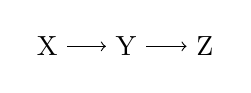
\begin{tikzpicture}
    \node (X) at (0,0)  {X};
    \node (Y) at (1,0) {Y};
    \node (Z) at (2,0) {Z};
    \path [->] (X) edge node {} (Y);
    \path [->] (Y) edge node {} (Z);
\end{tikzpicture}
\end{figure}

\begin{figure}[h]
\centering 
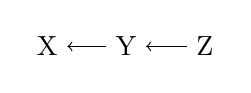
\begin{tikzpicture}
    \node (X) at (0,0)  {X};
    \node (Y) at (1,0) {Y};
    \node (Z) at (2,0) {Z};
    \path [<-] (X) edge node {} (Y);
    \path [<-] (Y) edge node {} (Z);
\end{tikzpicture}
\end{figure}

\begin{figure}[h]
\centering 
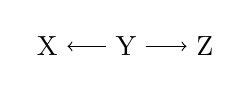
\begin{tikzpicture}
    \node (X) at (0,0)  {X};
    \node (Y) at (1,0) {Y};
    \node (Z) at (2,0) {Z};
    \path [<-] (X) edge node {} (Y);
    \path [->] (Y) edge node {} (Z);
\end{tikzpicture}
\end{figure}

WTS $X \perp Z|Y$

\begin{enumerate}
    \item The Markov Condition directly implies $Z \perp X | Y$ ($Z$ is independent of all nodes excluding its parents \{$Y$\} and descendants \{$\varnothing$\} conditioned upon its parents)
    \item $X \perp Z |Y$ again by Markov condition (same as above)
    \item Markov Condition again in a similar way wrt either $X,Z$ (both have empty set descendants, $Y$ as parent) 
\end{enumerate}

\subsubsection*{5}

\begin{figure}[H]
\centering 
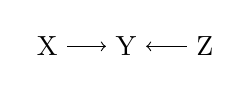
\begin{tikzpicture}
    \node (X) at (0,0)  {X};
    \node (Y) at (1,0) {Y};
    \node (Z) at (2,0) {Z};
    \path [->] (X) edge node {} (Y);
    \path [<-] (Y) edge node {} (Z);
\end{tikzpicture}
\end{figure}

Consider now the above DAG with a collider present, WTS $X \perp Z$ and $X \not\perp Z | Y$:  \newline  
  
$X\perp Z$ follows from Markov Condition ($Z$ is not a descendant of $X$, $X$ has no parental nodes) or noting that $X,Z$ are d-separated (specifically only when \textbf{not} conditioning on $Y$). \newline 

We know that $X \perp Z | Y \Leftrightarrow X, Z$ are d-separated. We note by definition $X,Z$ are d-connected conditioning on $Y$ and thus $X \not\perp Z | Y$. 

\subsubsection*{6}

{\textit Simulations omitted}

\begin{gather*}
    f_{X,Y,Z}
    =
    f_{Z|Y}f_{Y|X}f_X
\end{gather*}

\subsubsection*{7}

{\it DAG Omitted}

Consider the set of nodes $V = \{Z_j, X, Y_i\}$, $i,j=[4]$: 

\begin{gather*}
    f_{V}
    =
    f_X
    \prod_{k=1}^4
    f_{Z_k}f_{Y_k | Z_k, X}
%    f_{Z_1}f_{Z_2}f_{Z_3}f_{Z_4}
%    f_X
%    f_{Y_1 | Z_1, X}
%    f_{Y_2 | Z_2, X}
%    f_{Y_3 | Z_3, X}
%    f_{Y_4 | Z_4, X}
\end{gather*}

$X \perp Z_j, \forall j \in [4]$ follows directly from the Markov Condition, as no $Z_j$ is a parent or descendent of $X$. We could also note $X, Z_j$ collide at $Y_j$ and are d-separated, thus $X\perp Z_j$ but $X \not\perp Z_j | Y_j$ ($\forall j \in [4]$). 


\subsubsection*{8}

\begin{enumerate}[label=(\alph*)]
    \item 
    \begin{gather*}
        \Psymb(Z|Y)
        =
        \frac{ \sum_{x=0}^1 \Psymb(Z, Y, X=x)}
        { \sum_{x=0}^1 \Psymb(Y, X=x) }
        =
        \frac{ \sum_{x=0}^1 \Psymb(Z|Y, X=x)\Psymb(Y|X=x)\Psymb(X=x)}
        { \sum_{x=0}^1 \Psymb(Y, X=x) }
    \end{gather*}
    
    Result omitted, calculation follows from expression above (all information known from given information)
    
    \item Omitted 
    \item {\it Incomplete}
    \item Omitted   
\end{enumerate}



\subsubsection*{9}

\begin{enumerate}[label=(\alph*)]
    \item {\it Incomplete}
\end{enumerate}

\boxsection*[Chapter 18: Undirected Graphs]

\boxsubsection*{Questions, Definitions, Notes, Properties, etc.}

\begin{enumerate}
    \item Pairwise Markov property for $\mathcal{G}=(V,E)$,  $X,Y \subseteq V$, and $V\backslash\{X,Y\}$ is all nodes excluding $X,Y$:
    
    {\centering No edge exists between $X,Y \Leftrightarrow X \perp Y | V\backslash\{X,Y\}$ \par}


    \item The Global Markov states for sets of vertices $A, B, C \subseteq V$ in graph $\mathcal{G}$:   

    {\centering 
    $A \perp B | C 
    \Leftrightarrow $
    $C$ separates $A,B$
    \par}

    \item $M_\text{ pair}(\mathcal{G})
    =
    M_\text{global}(\mathcal{G})$
\end{enumerate}

\boxsubsection*{Exercises}

\subsubsection*{1}

\begin{figure}[H]
\centering 
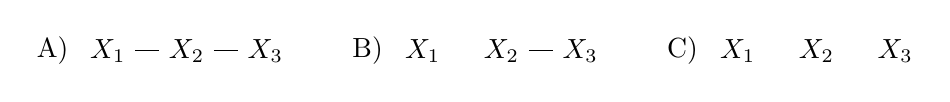
\begin{tikzpicture}
    %(a)
    \node (A) at (0.3, 0) {A)};
    \node (X11) at (1, 0) {$X_1$};
    \node (X21) at (2, 0) {$X_2$};
    \node (X31) at (3, 0) {$X_3$};
    \path [-] (X11) edge node {} (X21); 
    \path [-] (X21) edge node {} (X31); 

    %(b)
    \node (B) at (4.3, 0) {B)};
    \node (X12) at (5, 0) {$X_1$};
    \node (X22) at (6, 0) {$X_2$};
    \node (X32) at (7, 0) {$X_3$};
    \path [-] (X22) edge node {} (X32); 

    %(c)
    \node (C) at (8.3, 0) {C)};
    \node (X13) at (9, 0) {$X_1$};
    \node (X23) at (10, 0) {$X_2$};
    \node (X33) at (11, 0) {$X_3$};
\end{tikzpicture}
\end{figure}

All three relationships also hold trivially for the graph in (C). 

\subsubsection*{2}

\begin{figure}[H]
\centering
    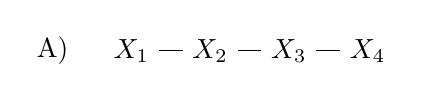
\begin{tikzpicture}
        \node (A) at (-1, 0) {A)};
        \node (X1A) at (0, 0) {$X_1$};
        \node (X2A) at (1, 0) {$X_2$};
        \node (X3A) at (2, 0) {$X_3$};
        \node (X4A) at (3, 0) {$X_4$};
        \path [-] (X1A) edge node {} (X2A);
        \path [-] (X2A) edge node {} (X3A);
        \path [-] (X3A) edge node {} (X4A);
    \end{tikzpicture}
\end{figure}


\begin{figure}[H]
\centering
    \begin{tikzpicture}
        \node (B) at (-1, 0) {B)};
        \node (X1B) at (0, 0) {$X_1$};
        \node (X2B) at (2, 0) {$X_2$};
        \node (X3B) at (1, -1) {$X_3$};
        \node (X4B) at (1, 0) {$X_4$};
        \path [-] (X2B) edge node {} (X4B);
        \path [-] (X4B) edge node {} (X1B);
        \path [-] (X4B) edge node {} (X3B);
    \end{tikzpicture}
\end{figure}



\begin{figure}[H]
\centering
    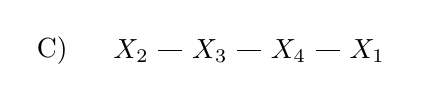
\begin{tikzpicture}
        \node (C) at (-1, 0) {C)};
        \node (X1C) at (3, 0) {$X_1$};
        \node (X2C) at (0, 0) {$X_2$};
        \node (X3C) at (1, 0) {$X_3$};
        \node (X4C) at (2, 0) {$X_4$};
        \path [-] (X2C) edge node {} (X3C);
        \path [-] (X4C) edge node {} (X1C);
        \path [-] (X4C) edge node {} (X3C);
    \end{tikzpicture}
\end{figure}

\subsubsection*{3}

\begin{enumerate}[label=(\alph*)]
    \item $X_1 \perp \{X_3, X_4\} | X_2; \\
    X_3 \perp X_4 | X_2$
    \item $X_1 \perp \{X_3, X_4\} | X_2$ or $X_1 \perp X_4 | X_3; \\ 
    X_2 \perp X_4 | X_3$
    \item $X_1 \perp X_3 | X_2, X_4; \\ 
    X_2 \perp X_4 | X_1, X_3$
    \item $X_1 \perp \{X_4, X_5, X_6\} | X_2, X_3; \\ 
    X_2 \perp X_6 | X_3, X_5; \ X_3 \perp X_4 | X_2, X_5; \\ 
    X_4 \perp \{X_3,X_6\} | X_2, X_5; \\ 
    X_6 \perp \{X_2, X_5\} | X_3, X_5$
\end{enumerate}

\subsubsection*{4}
\textit{Omitted }


    \iffalse 
        Consider $X_i \sim \text{Bernoulli}(p_i), i \in [3]$. Define $\Psymb(X_i=1, X_j=1) = p_{ij}$, noting that $X_i \perp X_j \Rightarrow p_{ij} = p_i p_j$. Under $H_0: p_{12|3} = p_{1|3}p_{2|3}$ and under $H_A: p_{12|3} \not=  p_{1|3}p_{2|3}$. 
        
        \begin{align*}
            \lambda 
            &= 
            \frac{
            \Psymb(X_1 = x_1 | X_3)
            \Psymb(X_2 = x_2 | X_3)
            }{
            \Psymb(X_1 = x_1, X_2 = x_2 | X_3)
            }
            \\
            &=
            \frac{
            p_{1|3}^{x_1} (1-p_{1|3})^{1-x_1}
            p_{2|3}^{x_2} (1-p_{2|3})^{1-x_2}
            }{
            asdf
            }
        \end{align*}
    \fi 

\subsubsection*{5}
\textit{Omitted}

\end{document}
